\section{The TGCT Tool}
TGCT is a cooperation platform for crowdsourced testing of Android application. As shown in Figure\ref{fig:arch}, TGCT works in the following process: (1) Building the GUI model of the application based on the automated testing process and the static analysis results of the GUI. It describes the jump between different windows corresponding to different events. (2) Taking test cases and uncovered window jumps as test tasks, the recommendation system predicts the preference of current crowd workers for test tasks based on the collaborative filtering recommendation algorithm. (3) According to the current window of crowd workers, the path from the window to the target test task is calculated. Taking a window jump as a unit, TGCT guides crowd workers to complete the path jump, reproduces the anomalies in automated testing or triggers new anomalies.
\begin{figure}[htbp]
\centering
\centerline{
\includegraphics[width=\columnwidth,height=4cm]{fig/2.png}}
\caption{The process of TGCT.}
\label{fig:arch}
\end{figure}

\subsection{Construction of GUI Model}
Building the GUI model of Android application is the basis of the implementation of the entire TGCT mechanism. Figure\ref{fig:flow_chart} shows the process of GUI model construction. Task requesters upload Android application APK on the crowdsourcing platform. TGCT parses APK from the perspective of automated testing and static source code respectively, and generates a GUI model for applications to be tested. The model includes three parts: normal window jump caused by events during automated testing, test cases that trigger exceptions, and uncovered window jump supplemented by static analysis for automated testing. These three parts will be described in detail in sections 2.1.1, 2.1.2 and 2.1.3.
\begin{figure}[htbp]
\centering
\centerline{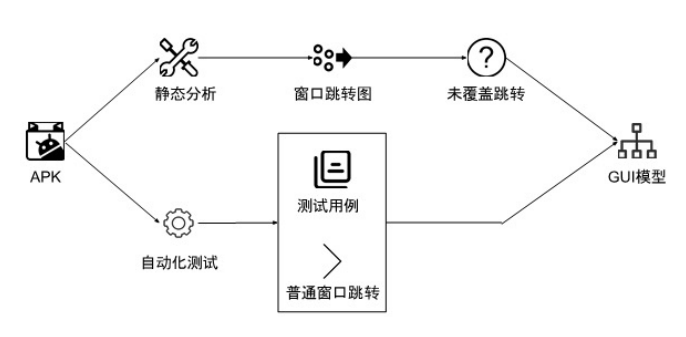
\includegraphics[width=\columnwidth,height=4cm]{fig/3.png}}
\caption{The process of GUI model construction.}
\label{fig:flow_chart}
\end{figure}

\subsubsection{Normal Window Jump}
This paper chooses the automated testing framework of MoocTest platform\footnote{www.mooctest.net}, uses depth-first search algorithm to traverse all components in the Android page, and assists with manual testing scripts. In the process of testing, the automated testing framework records the sequence of test events and saves screenshots before the test events occur. These screenshots are named timestamps and stored in the specified file directory. Based on the automated test results, TGCT stores the corresponding information of each test event in graph structure, and builds the GUI jump model of the application under test.

The automated testing framework records the sequence of events in the format of Figure\ref{fig:foramt}. The "time" field represents the time when the event occurred, and the "activityBeforeAction" field and the "activityAfterAction" field record the windows before and after the event, respectively. The "type" field represents the event type, and the "message" field outputs event information in detail. For different events, automated tests record event details in different formats.
\begin{figure}[htbp]
\centering
\centerline{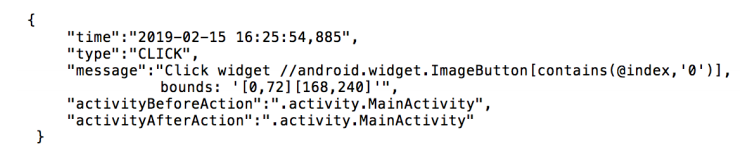
\includegraphics[width=\columnwidth,height=2cm]{fig/4.png}}
\caption{The format of event sequence.}
\label{fig:foramt}
\end{figure}

Traversing event sequences, TGCT stores GUI state changes recorded by automated tests in a directed graph structure: G = < N, E >, where N represents the set of points, which represents the set of Android application layer windows, and E represents the edge set, which represents the window jump set triggered by the event. 

The key storage fields of the edge are as follows: "source\_node" and "target\_node" store the names of start window and target window respectively, "event\_type" records event type, "event\_handlers" correspond to "message" in automated test events, "image\_URL" corresponds events to screenshots in the test process, and "message" field records events for triggering abnormal events. "create\_time" to save the time when the event occurred. TGCT sets the "data\_type" field to distinguish the window jump type in GUI model. Among them, 1 represents the normal window jump, 2 represents the test case triggering the exception, and 0 represents the uncovered window jump.

The automated test framework saves a screenshot of the current running state of the application,and names it with the current timestamp. The TGCT mechanism combines the coordinates of event-related components to mark the window components, assists in describing events, and provides clear test guidance. The processing of the screenshot information are as follows: (1) \textbf{Correspond screenshots to events:} Read the screenshots list P. For any screenshots $p_{i}$, whose file name is $n_{i}$, an edge $e_{i}$ can be found in the application edge set E. It satisfies the corresponding timestamp $t_{i}$, which is greater than $n_{i}$ and closest to $n_{i}$. The mapping relationship between $p_{i}$ and $e_{i}$ is established.
(2) \textbf{Associate user interaction events and corresponding screenshots:} an Android application contains multiple components, so how does TGCT describe the test event-related components to crowdsourced workers? On the one hand, for the user interaction test event, the TGCT draws the component in the screenshot according to the component coordinates recorded in the corresponding test event, then TGCT feeds it back to the worker. On the other hand, for the system test event, the TGCT does not modify the original screenshot, but just saves it.

\subsubsection{Test Cases}
The automated testing framework exports program run logs, each of which is formatted as shown in Figure\ref{fig:foramt2}. When the application starts, the Android system opens a new thread of execution for it, which generates other sub-threads and runs other windows of the application in the sub-threads. Threads are distinguished by thread ID as a unique identifier. In program log, thread ID is used as identifier to record resource loading process and program running status in different threads. The "type" field records the debugging information of the program log, the "LOG" field receives the information from the program's specific code, and the "time" field stores the timestamp generated by the exception. 
\begin{figure}[htbp]
\centering
\centerline{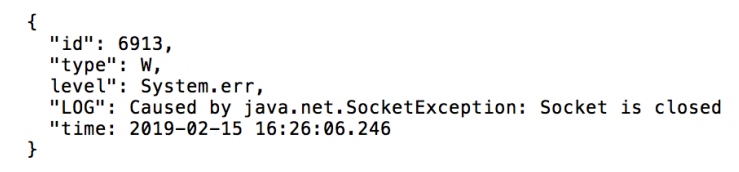
\includegraphics[width=\columnwidth,height=2cm]{fig/5.png}}
\caption{The format of program log.}
\label{fig:foramt2}
\end{figure}

For any log $l_{i}$ in the exception log set L, its corresponding time is $t_{i}$. In the edge set E, there must be an edge $e_{i}$, whose occurrence time is less than $t_{i}$ and closest to $t_{i}$. The TGCT mechanism searches for the corresponding event information for each exception log, modifies the window jump information, sets the "data\_type" field to 2, and outputs the "LOG" information in the log to the "message" field.

\subsubsection{Uncovered Window Jump}
Based on the work of Yang [49], Shengqiang [38] et al. developed a client tool GATOR, which generates window translation graph (WTG). The nodes in the graph are windows, including activities, menu and dialog. The callback information triggering window changes is recorded in the edge of the graph, and the information contained in each edge is shown in Figure\ref{fig:info}. The "source\_node" field and the "target\_node" field store the name of the starting node and the target node respectively. The "event\_handlers" field stores the window where the callback function occurs and the definition of the callback function. GATOR establishes the mapping between callback function and GUI interaction. By analyzing the name and definition of callback function, the event information corresponding to callback function is stored in the "type" field.
\begin{figure}[htbp]
\centering
\centerline{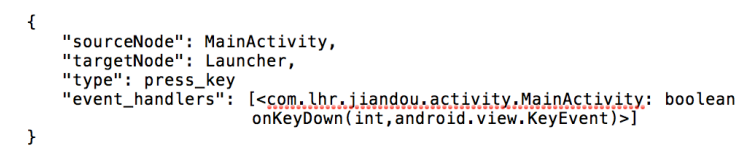
\includegraphics[width=\columnwidth,height=2cm]{fig/6.png}}
\caption{The information of edge in WTG.}
\label{fig:info}
\end{figure}

The TGCT mechanism traverses the edges of WTG, retrieves the event information of automated testing, and determines whether the window jump has been covered in the process of automated testing. If the window jump is not included, the TGCT mechanism stores the edge information from WTG in the format of normal window jump, and sets the "data\_type" field to 1. 

\subsection{Test Task Recommendation system}
The TGCT mechanism uses an item-based collaborative filtering algorithm to implement a test task recommendation system for test cases and uncovered windows. Cold start is a problem that must be faced by the collaborative filtering algorithm. Combining with GUI model in section 3.1, the mechanism of TGCT analyses the attributes of different window jumps and solves the problem of cold start of recommendation system. From the perspective of collaborative crowdsourcing, the TGCT mechanism achieves uniform recommendation for different testing tasks and optimizes crowdsourcing resource allocation by tracking the completion of different testing tasks. Figure\ref{fig:recomd} shows the process of the entire recommendation system. The design of the recommendation system will be described in detail in sections 3.2.1, 3.2.2 and 3.2.3 below.
\begin{figure}[htbp]
\centering
\centerline{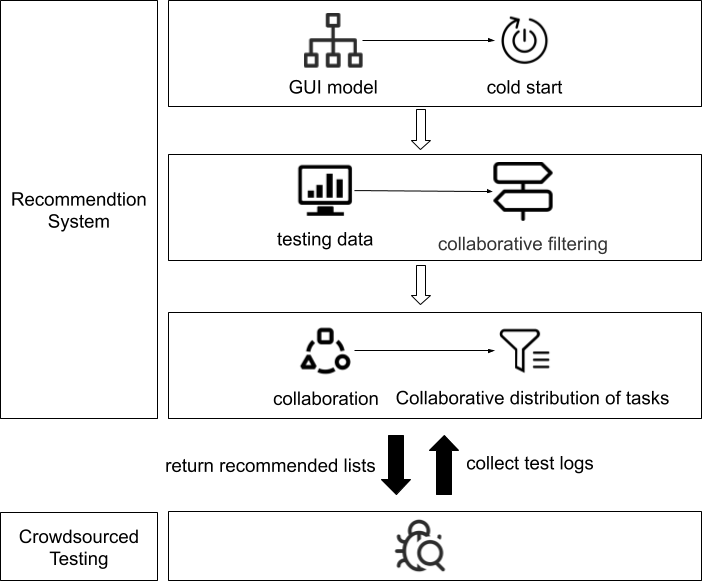
\includegraphics[width=\columnwidth,height=5cm]{fig/7.png}}
\caption{The process of the recommendation system.}
\label{fig:recomd}
\end{figure}

\subsubsection{Cold start}
In recommendation system for uncovered window jump, because uncovered window jump is difficult to find out the representative abnormal attributes, the TGCT mechanism adopts random strategy to solve the cold start problem. This paper mainly introduces the solution of cold-start problem of test case recommendation system from two aspects: cold-start for users and cold-start for items.

For new crowd workers, the recommendation system uses test data to solve the cold start problem. The steps are as follows:
(1)\textbf{Classification of anomalies:} Collect and understand the anomaly information in GUI model. TGCT mechanism classifies common anomalies in Android applications and manually evaluates the severity of anomalies. The higher the score, the more serious it is, as shown in Table\ref{fig:table33}.

\begin{table}[tb]
\caption{Common types and severity of anomalies in Android applications.}
\begin{center}
\begin{tabular}{|c|c|} %l(left)居左显示 r(right)居右显示 c居中显示
\hline 
Type&severity order\\
\hline  
Resource loading exception&6\\
\hline 
Input intent error&5\\
\hline 
Network exception&4\\
\hline 
ANR&3\\
\hline 
Thread exception&2\\
\hline 
Other exception&1\\
\hline
\end{tabular}
\label{fig:table33}
\end{center}
\end{table}
 
(2)\textbf{Anomaly selection:} According to the anomaly distribution of the current application, the TGCT mechanism randomly selects anomalies from each type to form test cases and recommend them to each new crowd worker.

So far, TGCT elaborates the solution of cold start problem for users, but the data is sparse and the recommendation effect is not good. Therefore, based on the solution of cold start problem for new users, the TGCT studies the solution of cold start for new items. The TGCT mechanism calculates the similarity between different test cases based on the cosine similarity by analyzing the properties of the anomaly, and realizes the coarse-grained personalized recommendation.

Based on the GUI model constructed in 3.1, TGCT describes test cases by three attributes. The test case $t_{i}$ is abstracted as a vector:
\begin{equation}
t_{i} = {(e_{1}, w_{1}),(e_{2}, w_{2}),(e_{3}, w_{3})}
\end{equation}

$e_{1}$ represents the exception type, and its corresponding weight $w_{1}$ is based on the severity of the exception defined in Table\ref{}. $e_{2}$ represents the start window of an exception, and its corresponding weight $w_{2}$ represents the page level of the window. For any window $w_{i}$, the corresponding page level $l_{i}$ is equal to the shortest path from MainActivity to $w_{i}$ plus 1. From the point of view of improving test coverage, the deeper the nesting of windows, the more difficult it is to detect abnormalities, and the higher the weight it gives, the more it is recommended to crowd workers. $e_{3}$ represents the event type, and the TGCT mechanism assigns different weights to different event types, as shown in Table\ref{fig:table34}.

\begin{table}[tb]
\caption{Event types and corresponding weights.}
\begin{center}
\begin{tabular}{|c|c|} %l(left)居左显示 r(right)居右显示 c居中显示
\hline 
Operation event type&Weight\\
\hline  
System event that acts on the phone button&1\\
\hline 
\tabincell{c}{User interaction events that \\act on program components in the phone screen}&2 \\
\hline
\end{tabular}
\label{fig:table34}
\end{center}
\end{table}

Test cases are represented by vectors, and the similarity $w_{ij}$ between test case A and test case B is calculated by cosine similarity in TGCT mechanism, where $A_{i}$ represents an attribute vector of test case A:
\begin{equation}
Similarity_{AB} = cos(\theta) = \frac{AB}{||A||||B||}
\end{equation}

\subsubsection{Item-Based Collaborative Filtering Recommendation}
The first five minutes of crowdsourcing testing is the cold start stage of the recommendation system. After collecting preference data of crowd worker, the recommendation system is completed by using the collaborative filtering algorithm based on items. Taking test cases as an example, given the test case set selected by the current crowd worker u, the preferences for other unselected test cases are calculated. The calculation steps are as follows: (1) \textbf{Compute the similarity between test cases:} The TGCT mechanism monitors the behavior of crowd workers and records the selection of different test cases by crowd workers. Based on the data, the similarity between different test cases is calculated. Similarity $w_{ij}$ between test case i and test case j are calculated using the following formula:
\begin{equation}
w_{ij} = \frac{|N(i) \cap N(j)|}{\sqrt{|N(i) \cup N(j)|}}
\end{equation}

N(i) denotes the group of workers who choose test case i to test, and N(j) denotes the group of workers who choose test case j to test. $N(i) \cap N(j)$ represents the crowd worker set that chooses both test case i and test case j. Among the crowd workers who choose test case i, the more workers choose test case j, the higher the similarity between test case i and test case j is.

(2) \textbf{Predict the preference of crowd workers for other test cases:} According to the historical test case set N(u) chosen by crowd workers u, the preference degree $p_(uj)$ of crowd workers u to test case j is predicted by TGCT based on KNN. The calculation formula is as follows:
\begin{equation}
p_{uj} = \sum_{i\in N(u) \cap S(j,k)}w_{ji}r_{ui}
\end{equation}

S(j,k) represents the set of k test cases closest to test case j. In the test case set N(u) which has been tested by crowd workers u, for each test case i, the similarity $w_(ji)$ between test case j and test case i is calculated. $r_(ui)$ represents the preference degree of crowd workers u for test case i. In the mechanism of TGCT, the value of $r_(ui)$ is between {0,1}. If crowd worker u chooses test case i, $r_(ui)$ = 1, otherwise, it is 0. 

(3) \textbf{Generate test lists in Top-N mode:} N test cases with the highest preference are selected and returned to the current crowd worker.

The recommended system for uncovered window jumps is the same above.

\subsubsection{Collaborative Test Task Assignment}
In Android crowdsourcing test with N participants, the TGCT mechanism defines the concept of "verified exception" for test case set T = {$t_{1}$, $t_{2}$,...}. In the crowdsourcing testing process, if a test case $t_{i}$ is tested more than the threshold S by crowd workers, its corresponding anomalies are considered to have been verified and will not appear in the recommended list. Recommendation system will guide crowd workers to verify and explore other anomalies, optimize crowdsourcing resource allocation, and improve the test coverage and efficiency.

\subsection{Real-time Guide Mechanism}
The TGCT is integrated into the mobile phone with Android SDK. Figure\ref{fig:guide} shows how the TGCT mechanism guides crowd workers to complete their testing tasks on the Android side. The TGCT judges the type of test task chosen by crowd workers. If it is a test case, it guides crowd workers to repeat abnormalities. If it is a jump from uncovered windows, it guides crowd workers to reach the starting window and explore new abnormalities.
\begin{figure}[htbp]
\centering
\centerline{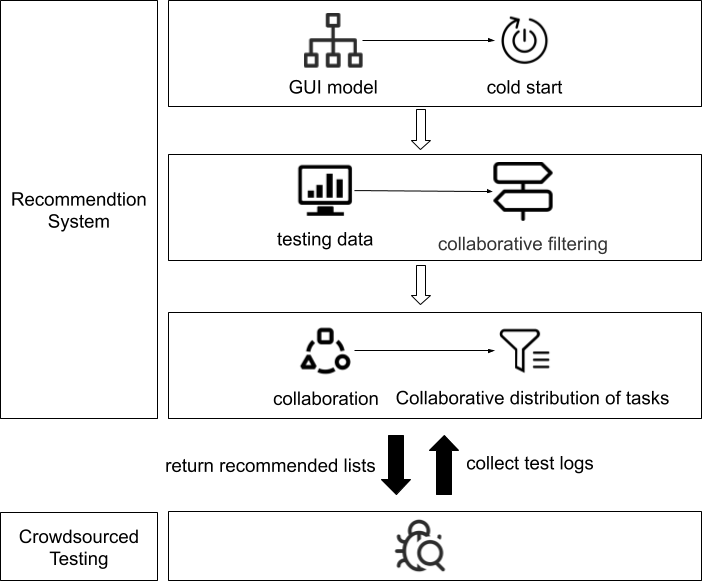
\includegraphics[width=\columnwidth,height=5cm]{fig/7.png}}
\caption{The process of the guide mechanism.}
\label{fig:guide}
\end{figure}

Real-time guide consists of two steps. First, the crowdsourcing worker is guided to reach the starting window of the target window jump from the current window. Secondly, for the test case, the TGCT guides the crowdsourcing worker to execute the operation event that triggers the exceptions in the starting window, and for the uncovered window jump ,TGCT mechanism prompts the crowdsourcing worker to complete the window jump event.The following will introduce the real-time boot design of the Android application from the jump path calculation and the real-time prompt.

\subsubsection{Jump Path}
There are three steps of calculating the jump path:
1. Remove the program's promotion window because these promotion window only face to new user and they are not meaningful.Start test from the MainActivity.
2. Construct an undirected graph based on the GUI model of step 1.
3. Calculate the shortest path through breadth-first traversal.
\subsubsection{Real-time Guidance}
According to the location information of crowd workers, the mechanism of TGCT chooses window jump according to different rules to realize real-time prompting and guidance. 
The status of crowd workers in the test path can be divided into the following categories:
1. The start window but not the start window of target window jump(edge).
2. The start window of target window jump(edge) but reached the first time.
3. The end window of target window jump(edge).

\begin{lstlisting}[ language=Java,caption={Algorithm: Shortest path calculation}]
    queue = currentWindow distance = 0
    While{queue is not empty do}{
        v = queue.poll();
        foreach edge in v.adjEdges do
            if edge.targetVertex.distance is MAXVALUE then              edge.targetVertex.distance = v.dist+1;
                queue = queue.offer(edge.targetVertex); edge.targetVertex.preVertex = v;
    }
\end{lstlisting}